%! TEX root = ../main.tex
% ============================================================
% IMMUTABLE — generated automatically, do not edit this block
%   script          : plotter.py
%   plot_type       : parallel_ratio
%   chapter         : 04
%   panel           : None
%   wind            : None
%   amplitude       : None
%   frequency       : None
%   probes          : None
%
% PANELS AVAILABLE:
%   FIGURES/04_parallel_ratio_allpanel-allwind-ampallamp-freqallfreq-probeallprobes.pdf
% ============================================================
\begin{figure}[htbp]
  \centering
  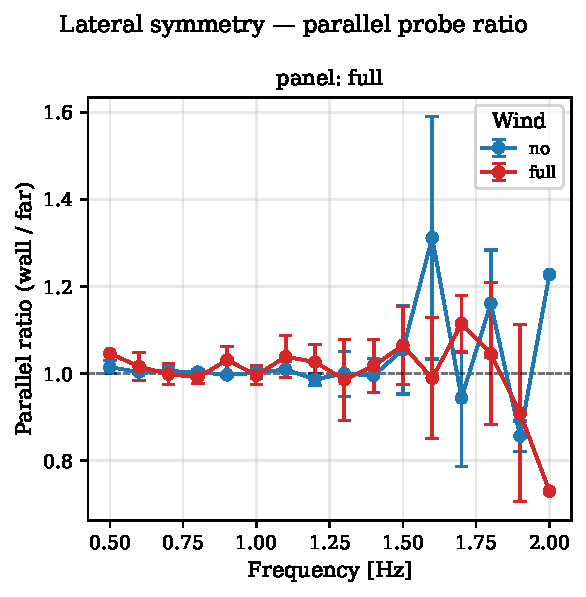
\includegraphics[width=0.9\linewidth]{FIGURES/04_parallel_ratio_allpanel-allwind-ampallamp-freqallfreq-probeallprobes.pdf}
  \caption[Ratio of wall-side to far-side probe amplitude at the same longitudinal distance, for 154 wave runs across 1 panel configurations]{
    Ratio of wall-side to far-side probe amplitude at the same longitudinal distance, for 154 wave runs across 1 panel configurations. A ratio of 1 indicates lateral symmetry. Deviations indicate wall reflections or wind-driven lateral asymmetry. Error bars: standard deviation across runs at the same frequency. Dashed line: ratio = 1.
  }
  \label{fig:ch04_parallel_ratio}
\end{figure}
